\documentclass{beamer}

% Solarized Theme
\usecolortheme[light, accent=orange]{solarized}
\beamertemplatenavigationsymbolsempty

% Packages
\usepackage[T1]{fontenc}
\usepackage[utf8]{inputenc}
\usepackage[english]{babel}

\usepackage{graphicx}
\usepackage{amsmath,amssymb,lmodern}
\usepackage{tikz}
\usepackage{tikzsymbols}
\usetikzlibrary{positioning, math, automata}
\usepackage{multicol}

\title{\Large{Annual Review}}
\author{Michalis Panayides}
\date{2020-06-10}

\begin{document}

\frame{\titlepage}
\begin{frame}
    \frametitle{Queues}
    \centering

    
\includegraphics[scale=0.3]{Bin/supermarket-queue.jpg}
    
\includegraphics[scale=0.3]{Bin/supermarket-queue.jpg}
    
\includegraphics[scale=0.3]{Bin/supermarket-queue.jpg}
\end{frame}


\begin{frame}
    \frametitle{Queues}
    \centering

    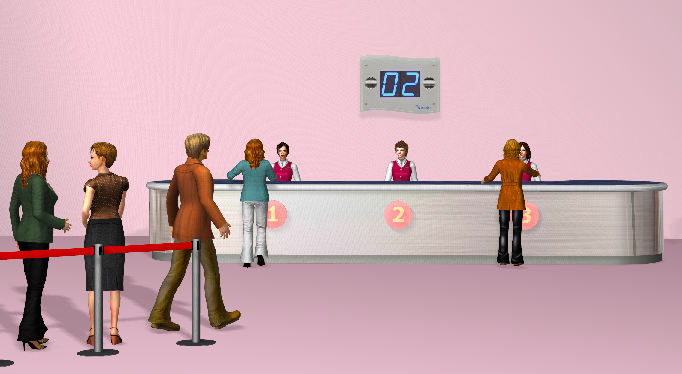
\includegraphics[scale=0.55]{Bin/bank-queue.png}
\end{frame}


\begin{frame}
    \frametitle{Queues}
    \centering
    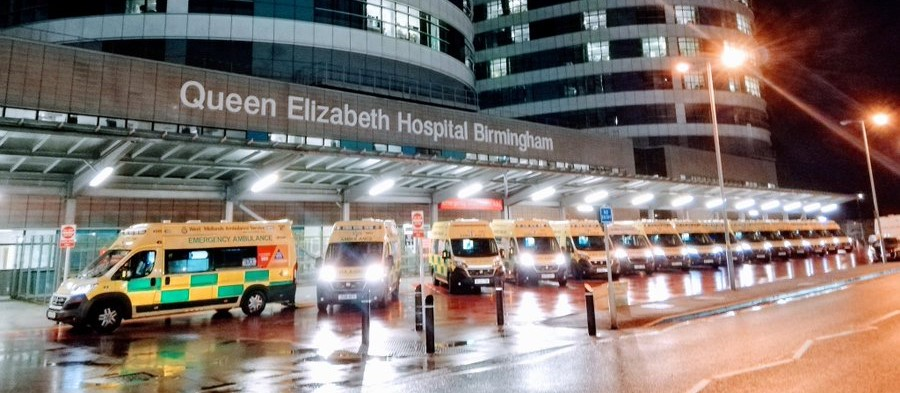
\includegraphics[scale=0.45]{Bin/ambulance_queue.jpg}
\end{frame}
\begin{frame}
    \frametitle{Queues}
    \centering

    
\includegraphics[scale=0.3]{Bin/supermarket-queue.jpg}
    
\includegraphics[scale=0.3]{Bin/supermarket-queue.jpg}
    
\includegraphics[scale=0.3]{Bin/supermarket-queue.jpg}
\end{frame}


\begin{frame}
    \frametitle{Queues}
    \centering

    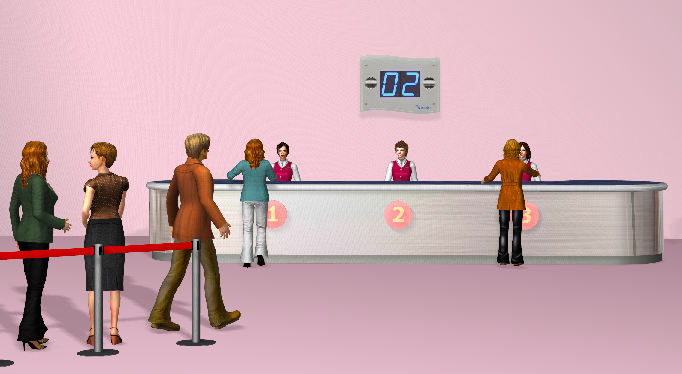
\includegraphics[scale=0.55]{Bin/bank-queue.png}
\end{frame}


\begin{frame}
    \frametitle{Queues}
    \centering
    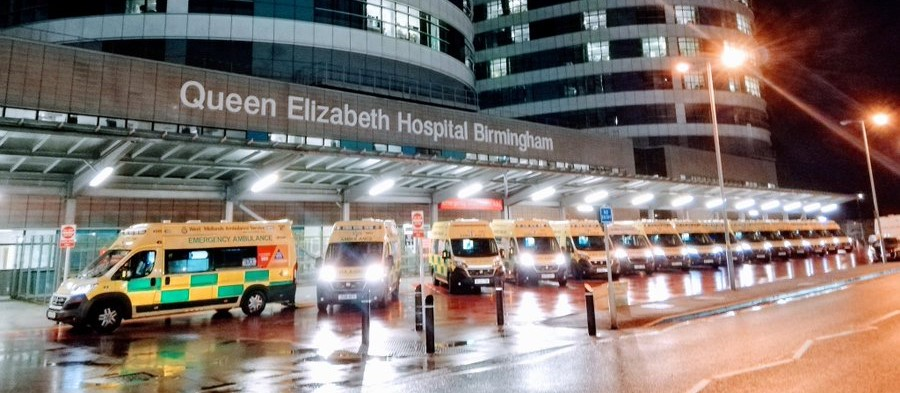
\includegraphics[scale=0.45]{Bin/ambulance_queue.jpg}
\end{frame}
\begin{frame}
    \frametitle{Queues}
    \centering

    
\includegraphics[scale=0.3]{Bin/supermarket-queue.jpg}
    
\includegraphics[scale=0.3]{Bin/supermarket-queue.jpg}
    
\includegraphics[scale=0.3]{Bin/supermarket-queue.jpg}
\end{frame}


\begin{frame}
    \frametitle{Queues}
    \centering

    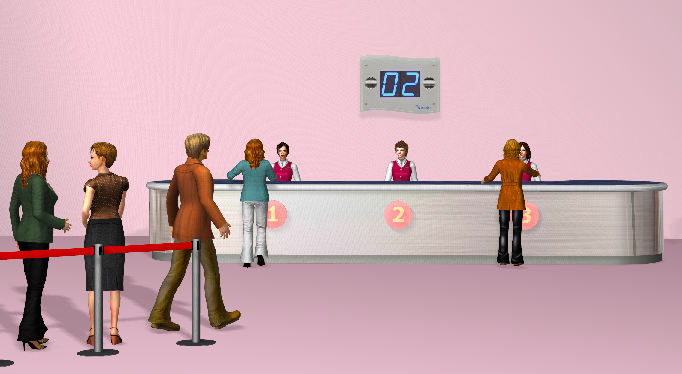
\includegraphics[scale=0.55]{Bin/bank-queue.png}
\end{frame}


\begin{frame}
    \frametitle{Queues}
    \centering
    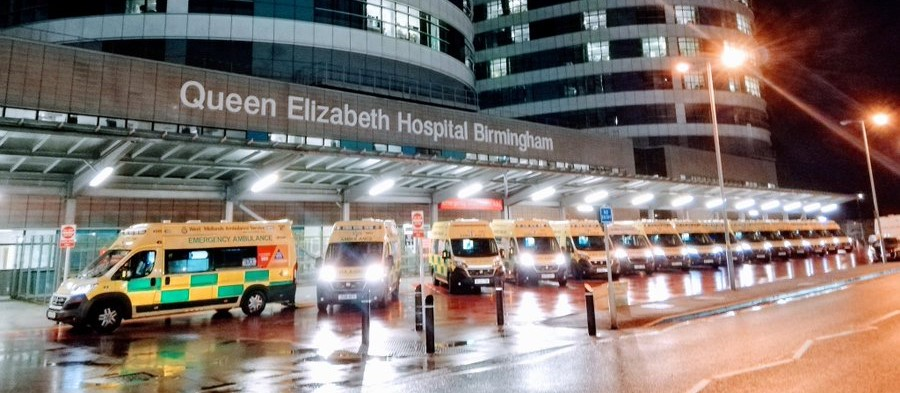
\includegraphics[scale=0.45]{Bin/ambulance_queue.jpg}
\end{frame}
\begin{frame}
    \frametitle{Queues}
    \centering

    
\includegraphics[scale=0.3]{Bin/supermarket-queue.jpg}
    
\includegraphics[scale=0.3]{Bin/supermarket-queue.jpg}
    
\includegraphics[scale=0.3]{Bin/supermarket-queue.jpg}
\end{frame}


\begin{frame}
    \frametitle{Queues}
    \centering

    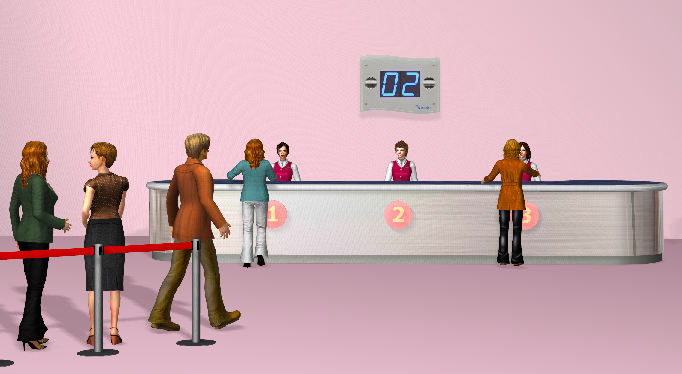
\includegraphics[scale=0.55]{Bin/bank-queue.png}
\end{frame}


\begin{frame}
    \frametitle{Queues}
    \centering
    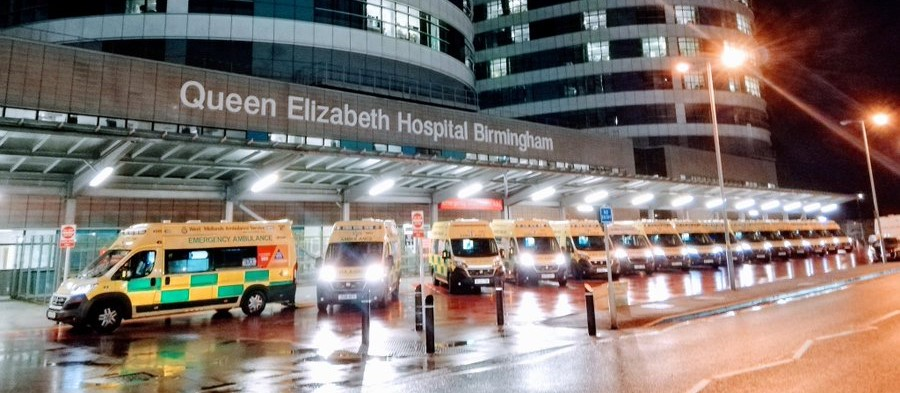
\includegraphics[scale=0.45]{Bin/ambulance_queue.jpg}
\end{frame}
\begin{frame}
    \frametitle{Queues}
    \centering

    
\includegraphics[scale=0.3]{Bin/supermarket-queue.jpg}
    
\includegraphics[scale=0.3]{Bin/supermarket-queue.jpg}
    
\includegraphics[scale=0.3]{Bin/supermarket-queue.jpg}
\end{frame}


\begin{frame}
    \frametitle{Queues}
    \centering

    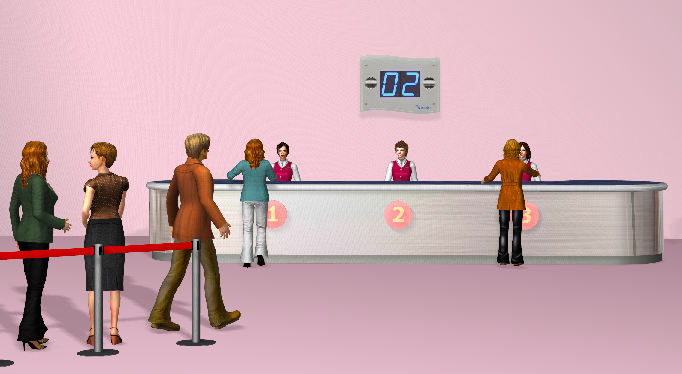
\includegraphics[scale=0.55]{Bin/bank-queue.png}
\end{frame}


\begin{frame}
    \frametitle{Queues}
    \centering
    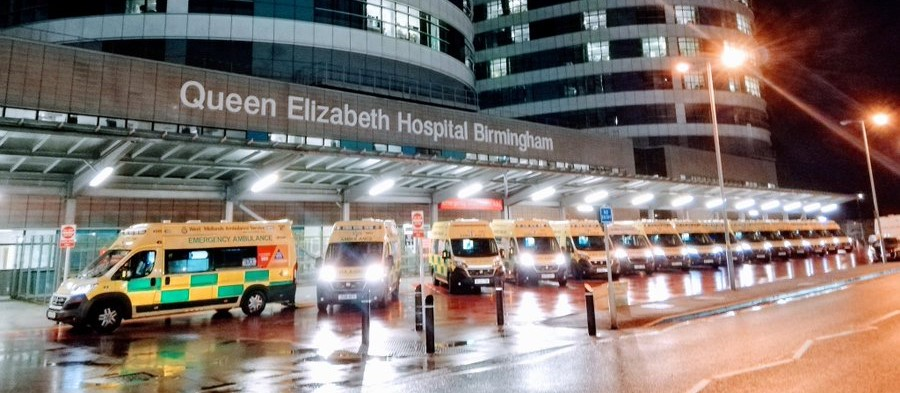
\includegraphics[scale=0.45]{Bin/ambulance_queue.jpg}
\end{frame}
\begin{frame}
    \frametitle{Queues}
    \centering

    
\includegraphics[scale=0.3]{Bin/supermarket-queue.jpg}
    
\includegraphics[scale=0.3]{Bin/supermarket-queue.jpg}
    
\includegraphics[scale=0.3]{Bin/supermarket-queue.jpg}
\end{frame}


\begin{frame}
    \frametitle{Queues}
    \centering

    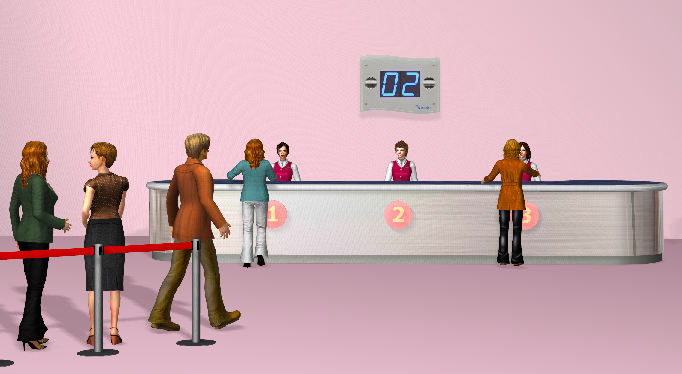
\includegraphics[scale=0.55]{Bin/bank-queue.png}
\end{frame}


\begin{frame}
    \frametitle{Queues}
    \centering
    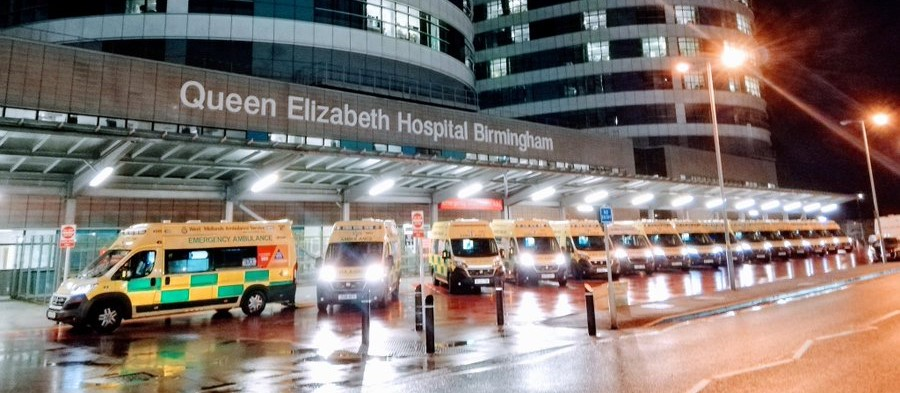
\includegraphics[scale=0.45]{Bin/ambulance_queue.jpg}
\end{frame}
\begin{frame}
    \frametitle{Queues}
    \centering

    
\includegraphics[scale=0.3]{Bin/supermarket-queue.jpg}
    
\includegraphics[scale=0.3]{Bin/supermarket-queue.jpg}
    
\includegraphics[scale=0.3]{Bin/supermarket-queue.jpg}
\end{frame}


\begin{frame}
    \frametitle{Queues}
    \centering

    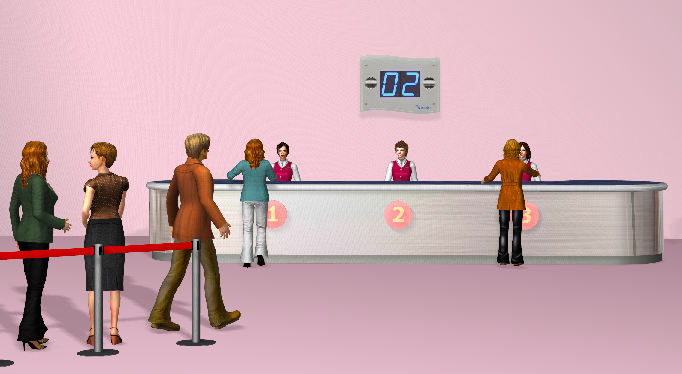
\includegraphics[scale=0.55]{Bin/bank-queue.png}
\end{frame}


\begin{frame}
    \frametitle{Queues}
    \centering
    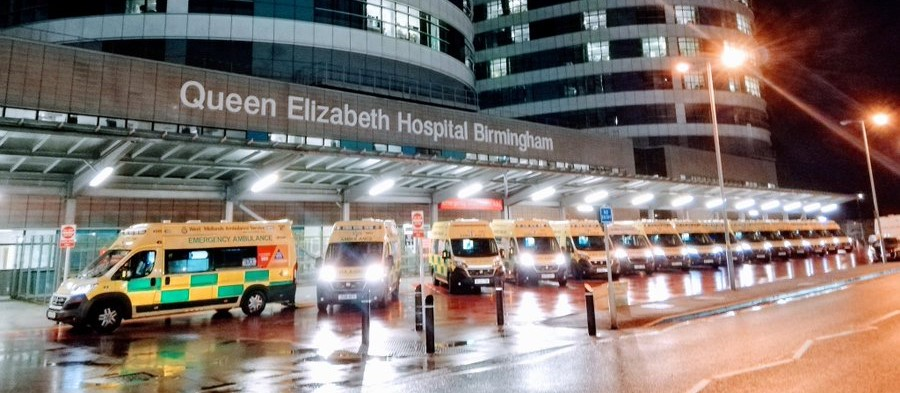
\includegraphics[scale=0.45]{Bin/ambulance_queue.jpg}
\end{frame}
\begin{frame}
    \frametitle{Queues}
    \centering

    
\includegraphics[scale=0.3]{Bin/supermarket-queue.jpg}
    
\includegraphics[scale=0.3]{Bin/supermarket-queue.jpg}
    
\includegraphics[scale=0.3]{Bin/supermarket-queue.jpg}
\end{frame}


\begin{frame}
    \frametitle{Queues}
    \centering

    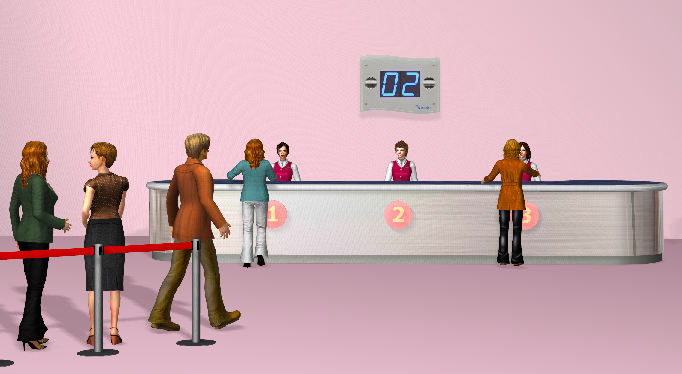
\includegraphics[scale=0.55]{Bin/bank-queue.png}
\end{frame}


\begin{frame}
    \frametitle{Queues}
    \centering
    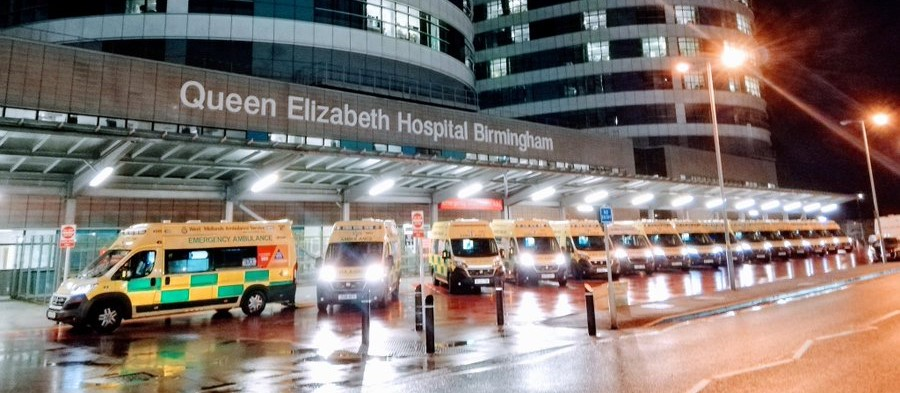
\includegraphics[scale=0.45]{Bin/ambulance_queue.jpg}
\end{frame}
\begin{frame}
    \frametitle{Queues}
    \centering

    
\includegraphics[scale=0.3]{Bin/supermarket-queue.jpg}
    
\includegraphics[scale=0.3]{Bin/supermarket-queue.jpg}
    
\includegraphics[scale=0.3]{Bin/supermarket-queue.jpg}
\end{frame}


\begin{frame}
    \frametitle{Queues}
    \centering

    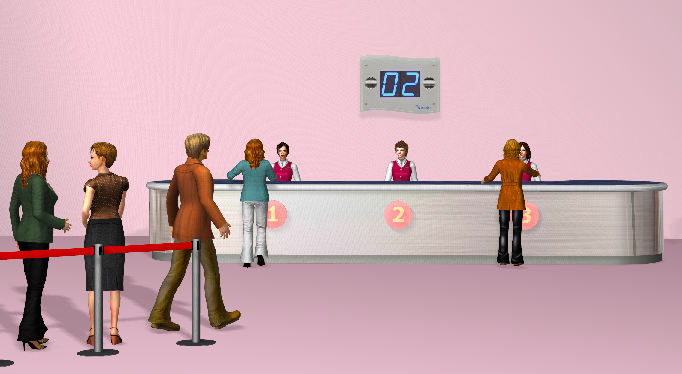
\includegraphics[scale=0.55]{Bin/bank-queue.png}
\end{frame}


\begin{frame}
    \frametitle{Queues}
    \centering
    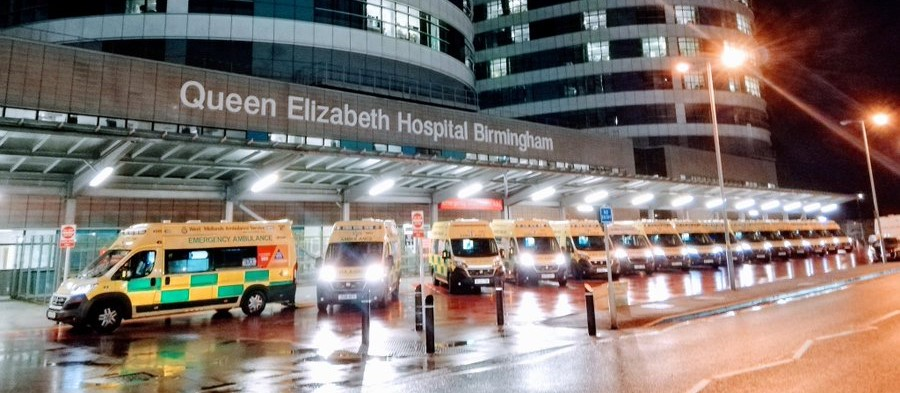
\includegraphics[scale=0.45]{Bin/ambulance_queue.jpg}
\end{frame}
\begin{frame}
    \frametitle{Queues}
    \centering

    
\includegraphics[scale=0.3]{Bin/supermarket-queue.jpg}
    
\includegraphics[scale=0.3]{Bin/supermarket-queue.jpg}
    
\includegraphics[scale=0.3]{Bin/supermarket-queue.jpg}
\end{frame}


\begin{frame}
    \frametitle{Queues}
    \centering

    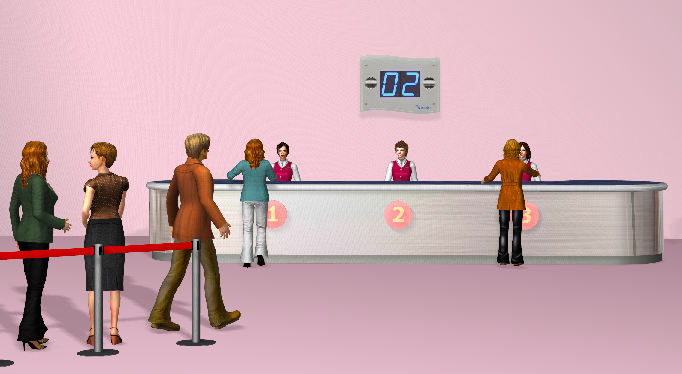
\includegraphics[scale=0.55]{Bin/bank-queue.png}
\end{frame}


\begin{frame}
    \frametitle{Queues}
    \centering
    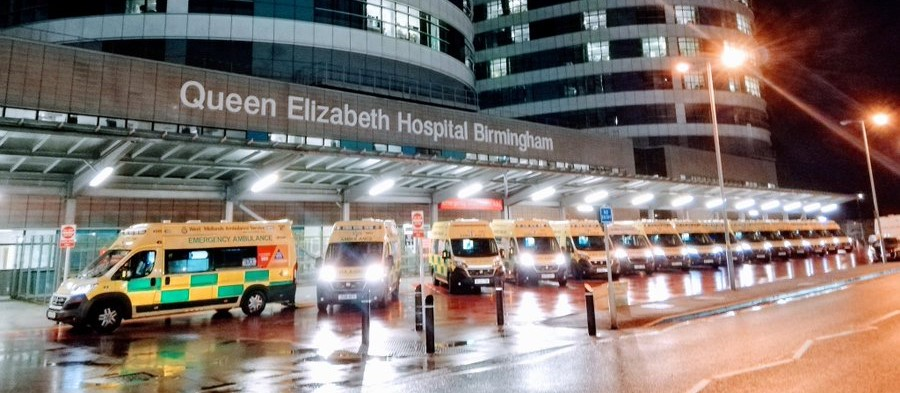
\includegraphics[scale=0.45]{Bin/ambulance_queue.jpg}
\end{frame}
\begin{frame}
    \frametitle{Queues}
    \centering

    \includegraphics[scale=0.3]{Bin/supermarket-queue.jpg}
    \includegraphics[scale=0.3]{Bin/supermarket-queue.jpg}
    \includegraphics[scale=0.3]{Bin/supermarket-queue.jpg}
\end{frame}


\begin{frame}
    \frametitle{Queues}
    \centering

    \includegraphics[scale=0.55]{Bin/bank-queue.png}
\end{frame}


\begin{frame}
    \frametitle{Queues}
    \centering
    \includegraphics[scale=0.45]{Bin/ambulance_queue.jpg}
\end{frame}
\begin{frame}
    \frametitle{Queues}
    \centering

    \includegraphics[scale=0.3]{Bin/supermarket-queue.jpg}
    \includegraphics[scale=0.3]{Bin/supermarket-queue.jpg}
    \includegraphics[scale=0.3]{Bin/supermarket-queue.jpg}
\end{frame}


\begin{frame}
    \frametitle{Queues}
    \centering

    \includegraphics[scale=0.55]{Bin/bank-queue.png}
\end{frame}


\begin{frame}
    \frametitle{Queues}
    \centering
    \includegraphics[scale=0.45]{Bin/ambulance_queue.jpg}
\end{frame}

% TODO: Iterative Removal: Highlight P1/P2
% TODO: Explain thoroughly games
% TODO: Magic dot on slide 39
% TODO: Change places of slides
% TODO: Make labels of graphs better
\end{document}